\section{Programación del NIOS II \label{sec:s1}}

\begin{center}
	\begin{minipage}{12cm}
		\begin{tcolorbox}[title=Actividad 1]
			Basado en el sistema creado en la práctica 6, crear un programa que mande valores al puerto paralelo (PIO) de 8 bits, cada 1 segundo. Investigar la función para escribir en el puerto y la función para crear un retardo.
		\end{tcolorbox}	
	\end{minipage}
\end{center}

En el entorno de programación del procesador Nios II, para escribir en un puerto de salida, generalmente se utilizan macros proporcionadas por el Sistema Operativo en Tiempo Real (RTOS) o por las librerías de hardware. La función más comúnmente usada es IOWR \cite{IO}, vista en la \autoref{prog:iowr}.

\lstinputlisting[
language=verilog,
label=prog:iowr,
caption={Utilización de la función ``IOWR''.}
]{
	codes/IOWR.c
}

Donde:
\begin{itemize}
	\item \textbf{BASE\_ADDRESS:} Es la dirección base del puerto de salida.
	\item \textbf{OFFSET:} Es el desplazamiento del registro específico dentro del puerto.
	\item \textbf{DATA:} Es el valor que se va a escribir en el puerto.
\end{itemize}

Para generar un retardo, se puede usar la función usleep (ver \autoref{prog:usleep}) que hace una pausa en la ejecución del programa durante un tiempo especificado en microsegundos. \cite{delay}

\lstinputlisting[
language=verilog,
label=prog:usleep,
caption={Utilización de la función ``usleep''.}
]{
	codes/usleep.c
}

Donde:
\begin{itemize}
	\item \textbf{TIME:} Es el número de microsegundos para el retardo.
\end{itemize} 

Primeramente, como se visualiza en la \autoref{fig:pinplanner}, se asignaron los pines de entradas y salidas del NIOS II en la tarjeta en donde se iba a implementar el procesador. Siguiendo los pasos indicados en la presentación, se utiliza la herramienta \textit{Eclipse} para generar un programa que imprima un mensaje en la consola, para ello se emplea una de las plantillas predeterminadas que ya trae el software. Una vez configurado el programa y construido el proyecto, se realiza la programación en la tarjeta, usando el puerto JTAG (ver \autoref{fig:programmer}) y al momento de ejecutar el proyecto en el hardware del NIOS II, se visualiza en la \autoref{fig:niosconsole}, el resultado en la consola.

\begin{figure}[ht]
	\centering
	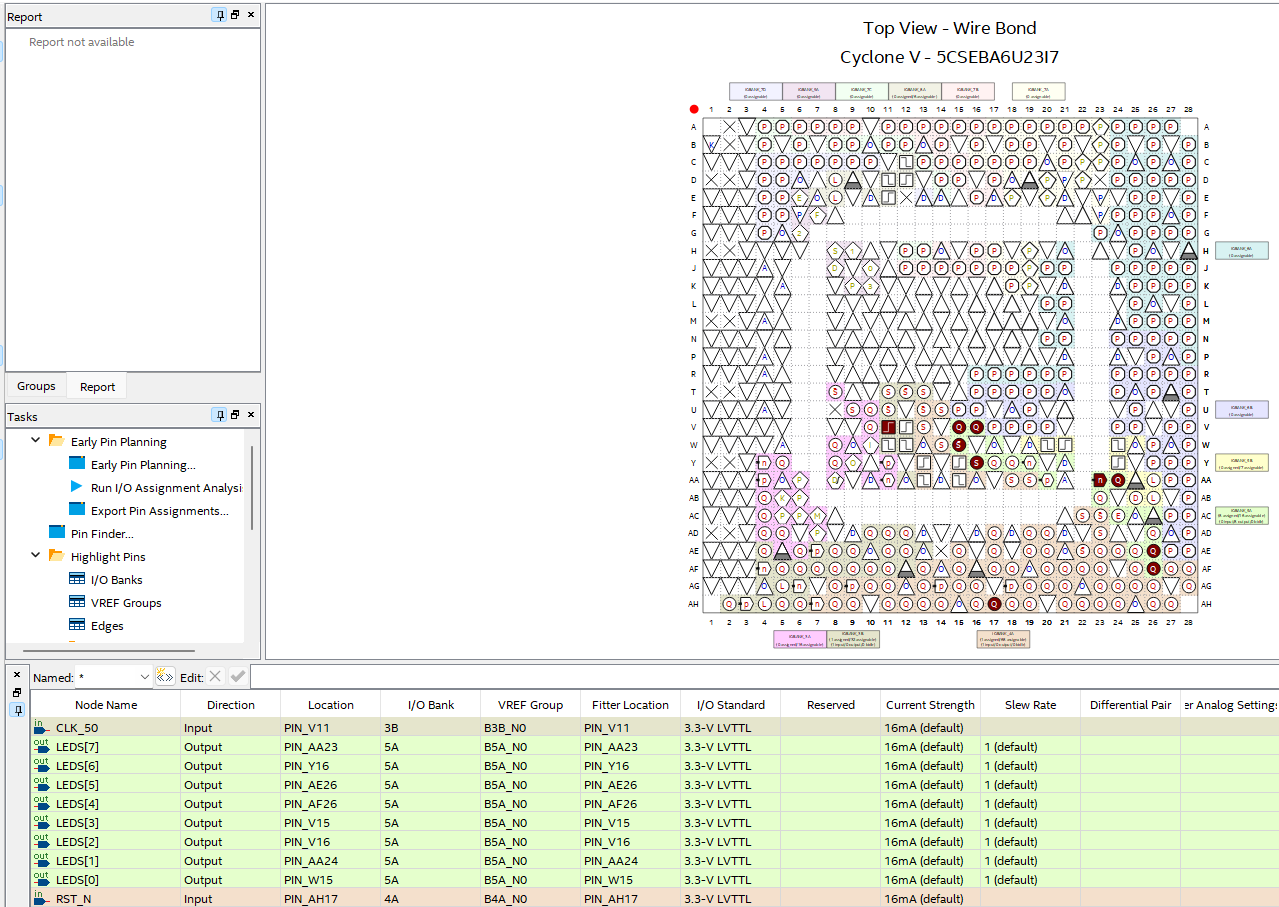
\includegraphics[scale=0.47]{PinPlanner.png}
	\caption{Asignación de los puertos de entradas y salidas procesador NIOS II en la tarjeta Cyclone V - 5CSEBA6U23I7. \label{fig:pinplanner}}
\end{figure}

\begin{figure}[ht]
	\centering
	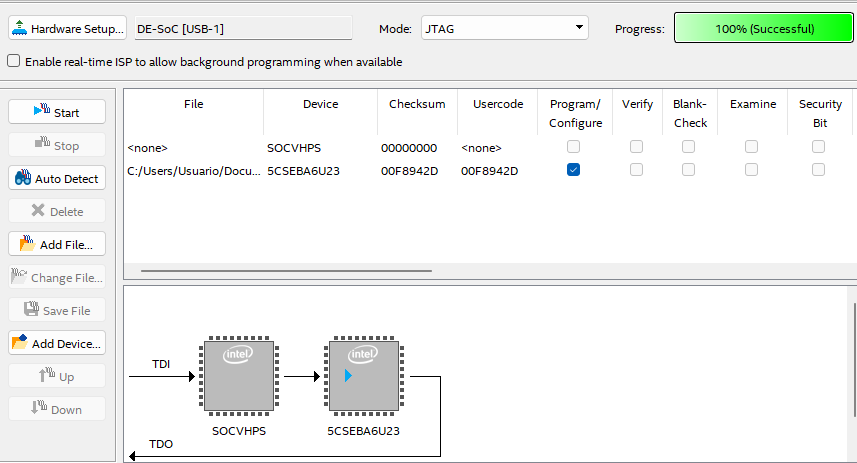
\includegraphics[scale=0.75]{Programmer.png}
	\caption{Programación del procesador NIOS II en la tarjeta Cyclone V - 5CSEBA6U23I7. \label{fig:programmer}}
\end{figure}

\begin{figure}[ht]
	\centering
	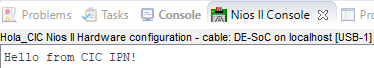
\includegraphics[scale=1.6]{NiosIIConsole.png}
	\caption{Resultado en la consola del Nios II. \label{fig:niosconsole}}
\end{figure}